\section{Introduction}

This thesis is about Social Weaving. A new technique that combines modern communication methods with existing web sites and web applications. The goal is to create a layer above the existing environment without directly modifying it. When we talk about "modern communication methods" we have social media in mind, like wiki pages, chats and comment boxes, but also support for file upload or appointment invitations to shared calendars. After all it doesn't matter what exactly is woven into the environment. Since it might be some HTML code, the user has the free choice. What is such an environment that we mentioned above? Informally we define an environment something that is visible through a browser. Now we have large variety of software we see in a browser. We have static and dynamic web pages, web applications using Flash or Java, and a lot of another technologies. The best case for Social Weaving would be to support seamlessly everything - but as we will see this is not possible.

\begin{figure}[!h]\centering
		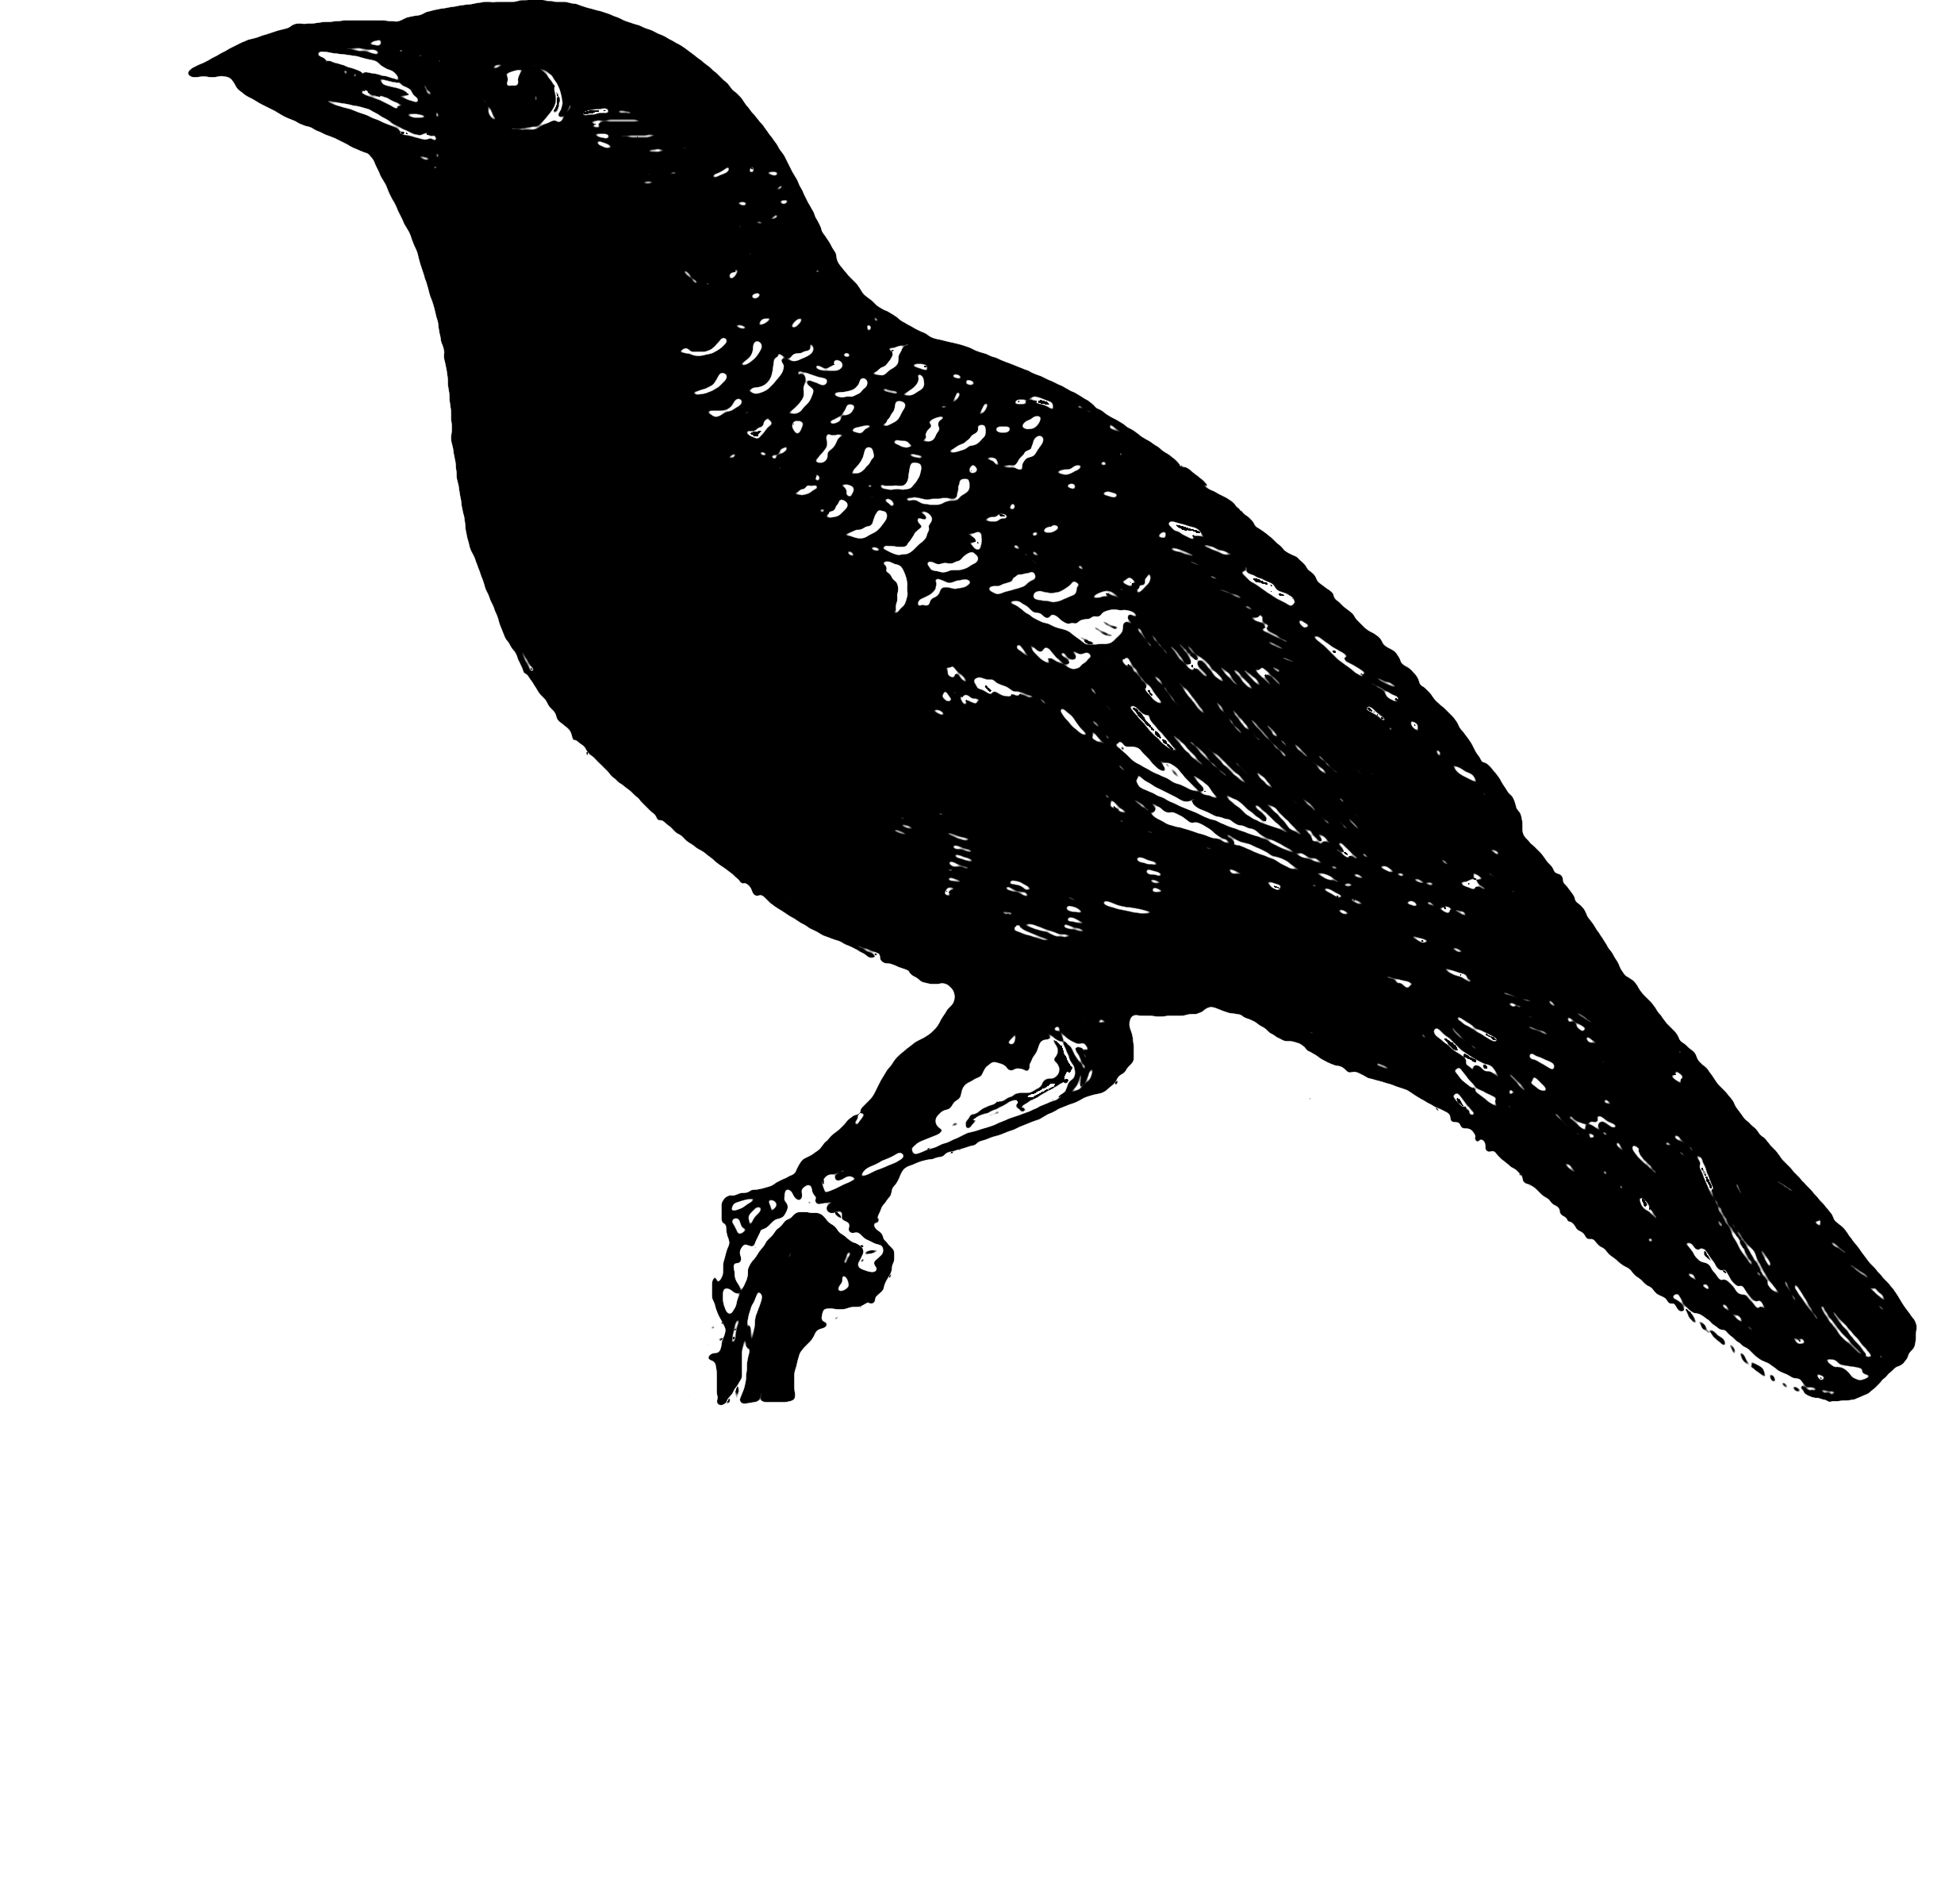
\includegraphics[width=5cm]{images/socialweaver.png}
		\caption{Social Weaver (Philetairus socius) is a species of bird in the Passeridae family endemic to Southern Africa}
		\label{socialweaver}
\end{figure} 

The great number of standards for the web doesn't prevent that every web page is constructed in a different way. There are no unique identifiers for elements, which would be necessary to guarantee a full Social Weaving support. Even though we cannot change the structures used in the web, we want to show what is possible with Social Weaving even now. 

In Section \nameref{contribution} - \ref{contribution} we discuss in detail how the basic idea of Social Weaving works and what problems it solves. The rest of this thesis is about Social Weaver - a prototype for Firefox that shows a basic functionality for certain environments. So the second part (\ref{sowe-reqs}) is an abstract requirement analysis that describes what a Social Weaving system needs. The third part (Section \ref{sowe-concrete}) shows the architecture of the prototype on a more concrete level.